\documentclass[a4paper]{article}

\usepackage[english]{babel}
\usepackage[utf8]{inputenc}
\usepackage{amsmath}
\usepackage{graphicx}
\usepackage[colorinlistoftodos]{todonotes}


%%%%%%%%%%%%%%%%%%%%%%%%%%%%%%

%Marija's packages
\usepackage{amsmath,amsthm,amsfonts,amssymb,amscd }
\usepackage{mathtools}
\usepackage{fullpage}
\usepackage{lastpage}
\usepackage{enumerate}
\usepackage{fancyhdr}
\usepackage{mathrsfs}

\usepackage{lineno,hyperref}
\usepackage{url}
\hypersetup{pdftex,colorlinks=true,allcolors=blue}

\usepackage{graphicx,setspace}
\usepackage{balance}
\usepackage{comment}
\usepackage{dblfloatfix}


\usepackage{fixltx2e}

%%%%
\usepackage[english]{babel}
\usepackage{cite}            % order citations
\usepackage{subfigure}      % several subfigures per figure environment

\usepackage{psfrag,color}
\usepackage{color}

\usepackage{graphics}

\usepackage{booktabs} 
\usepackage[boxed]{algorithm}
\usepackage{algpseudocode}

\usepackage{multicol}
\usepackage{multirow}
\usepackage{longtable}
\usepackage{capt-of}
\usepackage{array}
\usepackage{comment}

\usepackage{footnote}

\usepackage{tikz}
\usepackage{crmath}

% \newcommand{\todo}[1]{{\textcolor{red}{\textbf{TODO:} #1}}}
% \newcommand{\REVIEW}[1]{\texttt{\scriptsize{Hidden for review}}}
%\newcommand{\REVIEW}[1]{#1}

\usetikzlibrary{arrows, fit}

%%%%%%%%%%%%%%%%%%%%%%%%%%%%%%%%%%%%%%%%%%%%%%%

\title{\textbf{Context recognition for optimization of users' comfort in public buildings}}

\author{Marija Despenic}

\date{\today}

\begin{document}
\maketitle

\newpage

\tableofcontents
\newpage


\section {Introduction}

\subsection {Motivation for the work}		

\subsection {Problem description}

\subsection{Contributions}

\subsection{Thesis overview}

%%%%%%%%%%%%%%%%%%%%%%%%%%%%%%%%%%%%%
%%%%%%%%%%%%%%%%%%%%%%%%%%%%%%%%%%%%%
\section{Lighting preference profiles of users in an open office environment}\label{sec:PrefProfiles}

\color{red}This paper explains the motivation for the thesis - why personal control over lighting needs to be offered to the users, what kind of lighting profiles exist and why it is important to learn user preferences.
\color{black}
\\\\
In this paper we explain the following:
\begin{itemize}
	\item Offices in modern, commercial buildings are transforming into multiuser open office environments, or flex environments where people do not have predefined, personal desks. Nowadays, private offices are vanishing. Standards provide lighting recommendations to ensure comfortably lit office environments, but do not take into account that neighbouring users might differ due to their character, activity of preference. Providing all people satisfying lighting conditions becomes a challenge. 
	\item Several studies showed that broad range of individual lighting preferences exists, meaning that it is impossible to create satisfactory lighting conditions in multiuser environments by providing a fixed light level to all users. Therefore, personal control over lighting needs to be provided.
	\item There are several challenges in open plan environments:
	\begin{itemize}
		\item Due to the design practice for office lighting systems, multiuser environments are commonly deployed with a regular grid of luminaires that does not match the furniture layout. Therefore, in most cases, it is impossible to offer desk specific lighting in an open space office. A single luminaire would influence several neighbouring desks, thus the lighting conditions as well as lighting controls have a shared nature and are referred to as \textit{consensus control}. The common practice in such cases is to combine luminaires into control groups such that all luminaires in one control group act as one. Multiple users get shared control over the group of luminaires affecting their desks. 
		\item In the same control zone, the difficulties in finding consensus might be caused by differences in individual preferences. Influenced by the users’ character and sensitivity to light, a difference might also exist in how picky users are in their selection of preferred lighting. People have different personalities which can also influence how they interact with their environment in the office. Some people might be more dominant or vocal and feel less hesitation to express their preferences, while others might show a more submissive or conflict avoiding behaviour.  Due to differences between people occupying the same control zone, conflict between them might occur.
	\end{itemize}
\item Personal characteristics are believed to have an influence on users’ preferred and selected lighting, when given a choice. This paper presents insights gained from analysing light preference data of the users, obtained in two field studies. We show that users can be profiled based on their light preference and control behaviour in the following ways:
	\begin{itemize}
	\item \textit{Activeness} – The level of activity of each user can be determined based on the number of user control actions. The user’s control actions are a good basis to derive the user’s preference profile. Having only a few control actions of a user, makes derivation of user’s profile difficult. 
	\item \textit{Tolerance} – A tolerant user will select a broad range of illuminances meaning that he can work under a larger variety of lighting conditions. Contrarily, an intolerant user will demonstrate a more consistent preference for illuminance levels. When weighing users’ light preference profiles to offer satisfying lighting to multiple users, the tolerance of the users should be taken into account. The preference of an intolerant user asks for a higher weight, meaning that the proposed illuminance level should be shifted towards the light preference profile of the intolerant user. Users with a broad tolerance range will less likely experience conflict.
	\item \textit{Dominance} – Dominance is observed via the correlation between a particular user preferred illuminance level and the prevailing luminaire output in that zone. The dominance of a user is determined as a fraction of time the luminaire output matched the illuminance level set by that user. If the output of the luminaire is set according to the user’s preference for most of the time, the user is dominant in that control zone. Submissive (non-dominant) users are intimidated by others and manifest conflict avoiding behaviour, resulting in not changing the illuminance level even when dissatisfied.
	\item \textit {Preference} – The preference of a user is the control setting that is most comfortable for that user, leading to the highest user’s satisfaction with lighting conditions. Having opposing lighting preferences in one control zone might introduce dissatisfaction of the users and pose a risk of conflict.
	\end{itemize}
\item In this paper we propose a method for modeling lighting preference profiles of users and how they can be classified based on their activeness, tolerance, dominance and preference. Furthermore, we show that control zones can be classified based on lighting preference profiles of the users who occupy them, and the zone luminaire output. Analysing different types of user combinations in the control zones and the actions they performed to set their preferred lighting conditions, we can distinguish 3 cases:
	\begin{itemize}
		\item Case 1: All users in a control zone are satisfied, the probability of conflict occurring is low.
		\item Case 2: User(s) in a control zone are dissatisfied, the probability of conflict occurring is high.
		\item Case 3: User(s) satisfaction and the probability of conflict occurring is unknown and therefore, additional input from the user(s) is needed.
	\end{itemize}
We propose a method for zone classification as well and how we can properly request additional information when case 3 is detected.

\item \underline{Why we want to know the preference profiles of the users?} The results showed that there is a significant difference between lighting preference profiles of the users that needs to be taken into account when offering lighting conditions in open space environments. By knowing lighting preference profiles of the users and zone classification, satisfaction of the users can be improved by 
	\begin{itemize}
		\item Predicting the conflict between the users in the same control zone and facilitate in making a consensus control choices.
		\item Offering lighting conditions that meet the preference and the profiles of the users. A proposed light level should be a weighted combination of user profiles by taking into account whether users in the same zone are tolerant or intolerant. A tolerant user can be satisfied with broad range of light levels and therefore, the weighting should be done by shifting a proposed light level towards a preference of an intolerant, pickier user.  
		\item Triggering submissive users to express their preferences. A submissive user will represent an inactive user, whose choices are not correlated with the prevailing luminaire output in his zone. This situation might lead to increased discomfort of a user. In that case, additional user input should be required in order to derive his lighting preference profile as accurate as possible.
	\end{itemize}
\item Limitations of the current work and possible improvements (introduction to the future work):
	\begin{itemize}
	\item In these studies, individual presence information of users was not available. Lighting was controlled based on overall occupancy of the office space. Therefore, it was not possible to determine what each user actually experienced during the study, regarding lighting conditions. Having the presence information would help to generate the preference labels more accurately and to better distinguish between user’s preference and acceptance. An illuminance level set by a particular user is clearly recognizable as his preference. If a user experiences an illuminance level set by his zone neighbours, the presence of his colleagues influences the interpretation of this data. If a user is alone in a control zone, without any social obstacles to change lighting, the illuminance level of the zone represents the user’s preference, regardless of the action holder. If a user is not alone, the prevailing illuminance level represents the user’s acceptance, but might not be his preference. Distinguishing between acceptance and preference helps to recognize submissive users. If lighting conditions that user accepts differ from this user’s preference, this is an indication of submissiveness.
	\item Another problem that might arise from lack of individual presence information is that a group action as a result of an agreement between multiple users would be used as input to determine the preference of the user who performed the action. Without individual presence information, this action with be identified as a preferred choice of that user. 
 \color{red} Therefore, these were the reasons for setting up another study in 2016, where presence of each user can be derived based on motion sensors data. In that study, a field of view of each sensor was bounded to individual user's desk, providing the presence information of a specific user, rather then for the whole space. \color{black}
	\item In this paper, preference labels are derived based only on user’s lighting control actions and luminaire output data, and are independent from contextual and environmental data. Using this method, preference profiles could be determined without additional sensorial data. However, people could have different preference depending on e.g. the time of the day, weather conditions and presence of colleagues in the control zone or office space. Besides, when a user, for example, selects dimming levels in the ‘dark’ range, it might be that he does not prefer dark lighting conditions, but he compensates for high room brightness due to high wall luminance. Further elaboration on environmental factors that might influence user’s lighting preference should be performed (finding a 'real' preference function).  In that case, offering satisfactory lighting conditions can be done based on the current contextual information and it is assumed to be more accurate.
	\item In this paper the activeness is determined based on a proposed threshold of 2 actions per user. It is arguable whether reliable classification needs more data points. Additional evaluation is needed to assess the error in profiling based on this limited number of actions. However, with a higher threshold for activeness, the proposed method stays identical, only more users might be asked for additional satisfaction data, resulting in more reliable classification.
	\end{itemize}
\end{itemize}


This paper is based on the data from Study 2013 and 2014.  
 \color{red}(This paper is submitted to Building and Environment journal on August 24.) 

%%%%%%%%%%%%%%%%%%%%%%%%%%%%%%%%%%%%%%%%%
%%%%%%%%%%%%%%%%%%%%%%%%%%%%%%%%%%%%%%%%%
\color{black}
\section{Environmental factors that  influence users' comfort and preference}
%%%%%%%%%%%%%%%%%%%%%%%%%%%%%%
\subsection{Features that influence users' comfort} \label{sec:FeaturesUserComfort}

We want to find which features have the biggest influence on user's comfort.
\\\\
Assumption: User will react when he is dissatisfied with environmental conditions in order to restore his comfort. We want to predict under which environmental conditions user will react.  By knowing which states are causing discomfort of a user, we can try to avoid them. For example, if illuminance level (lux at user's desk) is one of the influential features, we can control lighting or blinds, to avoid user actions i.e. user's discomfort caused by certain states. We assume that at the moment $t$ user reacts to override conditions at $t-1$. This is posed as a classification problem:
\begin{equation}
class(t) = 
\begin{cases}
0 & \text{user didn't react under env. conditions at (t-1) }\\
1 & \text{user reacted under env. conditions at (t-1)}\\
\end{cases}
\end{equation}
\\\\
Goal: find the best, predictive features that will help to predict whether user will react or not. Why we want to do feature selection instead of taking all features? If we assume that feature is predictive, but in fact is irrelevant one, the prediction of user actions will be poor. Therefore, we want to find the most predictive ones. It will help us to find what influences user's comfort the most e.g. there is a lot of daylight increasing the glare, blinds are down and it is too dark etc. and therefore, user reacted. Features that influence user's comfort indirectly influence user's preference as well (there are states that cause user's discomfort and that should be avoided vs. states that user prefers).  Finding relevant features will also define the environmental sensors that need to be either embedded or connected to the lighting system. That would decrease installation and commissioning costs as well. 
\\\\
Before we try to do feature selection, we need to be able to predict user's actions. Otherwise, feature selection is meaningless. 
\\\\
Problem: User's actions are rare events. In our study, users had only a few control actions. This results in many points where users didn't react (a lot of 0s) and a few points where users reacted (few 1s), introducing the class imbalance problem in classification. Imbalance class problem exist in a situation when the number of instances of one class is much lower than the number of instances of another class.  Usually, underrepresented minority class represents the class of interest (positive class - class 1 ("user reacted") in our case) and since the most classifiers are designed to minimize the global error rate, they tend to classify all the instances as negative (belonging to the majority class).
\\\\
\color{red} This means that we first need to solve class imbalance problem, and then to do the feature selection. This motivates introduction of the two new algorithms for class imbalance problem explained in the next section.

%%%%%%%%%%%%%%%%%%%%%%%%%%%
\color{black}
\subsubsection{New cluster-based approaches for class imbalance problem}\label{sec:NewAlgos}

This paper is motivated by the fact that we cannot predict user's actions due to the class imbalance. Therefore, we also cannot find the features which have the highest influence on users' comfort. 
\\\\
In order to solve this problem, we introduced two new algorithms: \textit{Cluster-based oversampling + Tomek links and Cluster-based SMOTE oversampling + Tomek links}.
\\\\
The envisioned outline of the paper is the following:
\begin{enumerate}[I]
\item \textbf{Introduction}\\
In Introduction, we give an explanation why class imbalance problem is an important problem in classification domain. We give examples in real-life applications to motivate our work. We introduce the categorization of the algorithms developed so far for class imbalance problem (\textit{data level approaches, algorithm level approaches} and \textit{cost-sensitive methods}) and explain the differences between them. We introduce ensemble of classifiers and motivation behind using ensembles over single classifier in our approach. We enumerate our contributions:
\begin{itemize}
\item We introduce two new cluster-based algorithms for class imbalance problem and briefly explain motivation behind them.
\item We design experimental framework to analyse performance of 13 different algorithms developed for class imbalance problem that proved to perform the best in different domains and compare their performances with our algorithms. 
\item We show that our algorithm(s) outperforms the others. 
\end{itemize}
\item \textbf{Introduction to class imbalance problem}\\
In this section we introduce the nature of  class imbalance problem and explain why learning from imbalanced data sets might be difficult. We further present proper measures for performance evaluation of the classifiers in imbalanced domains. 
	\begin{enumerate}[1.]
	\item \textbf{The nature of class imbalance problem}\\
	There are several studies that showed that the skewed prior distribution of classes is not the major problem that hinders the performance of the classifiers. Rather, the class imbalance may yield to the following problems:
		\begin{enumerate}
		\item \textit{Small sample size}
		\item \textit{Overlapping between classes}
		\item \textit{Within-class imbalance and small disjuncts}
		\end{enumerate}
We present each of these problems and explain how they hinder the performance of classifiers.
	\item \textbf{Performance measures in imbalanced domains}\\
In this section we represent the proper measures for evaluation of classifier performance in imbalanced domains. We show why accuracy and error rate are not good measures. We introduce the concept of ROC (Receiver Operating Characteristic) curves and explain how ROC curves are consistent for a given problem even when distribution of classes is highly skewed. In order to compare performance of different classifiers, the area under a ROC curve (AUC) is commonly used. We explain why this is a good performance measure, how is calculated and what is statistical meaning of it. 
	\end{enumerate}

\item \textbf{Representative techniques for class imbalance problem}\\
In this section we introduce representative techniques for class imbalance problem that proved to perform the best in different domains. We explain the motivation behind of use the ensemble of classifiers over single classifier and what are the advantages of that approach. We introduce \textit{Bagging} and \textit{Boosting} as the most widely used ensemble based methods and explain how they assure the diversity in classifiers. We categorize the investigated methods in the following categories.
		\begin{enumerate}[I]
		\item Data level approaches
			\begin{enumerate}[1.]
			\item Sampling methods \\
			- Random oversampling\\
			- Random undersampling\\
			- Synthetic minority oversampling technique (SMOTE)\\
			- Cluster-based oversampling\\
			- Cluster-based undersampling\\
			- Cluster-based synthetic oversampling\\
			\item Cleaning methods\\
			- SMOTE + Tomek links\\
			- SMOTE + ENN
			\end{enumerate}
		\item Algorithm level approaches
			\begin{enumerate}[1.]
			\item Boosting-based ensembles \\
			- AdaBoost.M1\\
			- RUSBoost
			\item Bagging-based ensembles\\
			- UnderBagging\\
			- OverBagging \\
			- SMOTEBagging
			\end{enumerate}
		\end{enumerate}
We explain main advantages and drawbacks of enumerated algorithms and based on that motivate our work.

\item \textbf{New algorithms}

In this section we introduce two new algorithms and motivation behind them based on advantages and drawbacks of enumerated algorithms. The proposed two algorithms are hybrid algorithms that combine sampling and cleaning methods in order to increase the performance of classification. They simultaneously solve both, the problem of small disjuncts and overlapping between classes.
Why our algorithms might be better than others?
\begin{itemize}
\item \textit{Cluster-based oversampling + Tomek links}. Cluster-based oversampling solves not only between-class, but also within-class imbalance that might occur due to small disjuncts. Briefly, the $K$-means algorithm is performed in order to find the number of clusters in each class and both, majority and minority class clusters are randomly oversampled to reach the same number of instances. Tomek links solve the problem of overlapping between classes by removing the closest instances in both classes that are at the borderline, leading to well-defined clusters. 
\item  \textit{Cluster-based SMOTE oversampling + Tomek links}. Instead of using simple random oversampling to balance the number of instances in clusters of each class, we perform SMOTE oversampling to increase the diversity of instances and to solve the problem of overfitting that might occur by random oversampling. The problem with SMOTE oversampling is that may introduce artificial samples of one class to spread further in opposite class space, causing overlapping between classes. Again, Tomek links are combined with this approach to prevent class overlapping.  
\item This approach belongs to data level approaches, which have the main advantage of being independent on classification algorithm, in comparison to algorithm level approaches which request algorithms modification, meaning expert knowledge on each of them. Also, costs do not have to be inferred as in cost-sensitive methods. 
\item Cluster-based approaches cluster data based on similarity measures, meaning that we will populate different parts of the data space equally by balancing number of minority and majority class instances in the neighbourhood of each instance.
\end{itemize}
Here we also present the pseudo code of the two new algorithms and explain steps.

\item \textbf{Experimental framework}

We test before mentioned approaches, together with our two new algorithms on 15 publicly available data sets obtained from UCI Machine learning repository.
Here we present the overview of the data sets used with their number of instances, number of features, feature types etc. These data sets are approximately balanced i.e. with imbalanced ratios (IR) of approx. 1.
\\\\
We imposed class imbalance problem by altering the percentage of the positive instances from 10\% up to 50\% (balanced data set where each class contributes with approximately 50\% of instanced to the data set), with the step of 5\%. Why we do that? In most  papers, authors took imbalanced data sets and balanced them with mentioned algorithms. In that case, the algorithms are tested for only one case of imbalance ratio. By altering the percentage of imbalance (imbalance ratio) we want to see how each of these algorithms perform in general, when different imbalanced ratios are presented. This helps us to get better insight in general performance of each algorithm. Also, due to diversity of features that defined both classes in each data set, we assumed that each of these classes can represent the minority class.
\\\\
Parameter estimation - In our approach we use Random Forest as a base algorithm, except in boosting-based algorithms where we use ensemble of decision trees due to algorithms requirements. Therefore, we need to estimate the following parameters: optimal number of trees and minimum number of observation per tree leaf. We want to give the same opportunity to all algorithms to perform their best results, without fine tunning their parameters based on a data set. Therefore, we tested each algorithm for different number of trees: from 2  to 512, doubling the number of trees in each test (from $2^{1}$ until $2^{9}$). Also, the minimum number of instances per leaf is tested for 1, 5 and 10, taking 10 instances per leaf as the upper limit due to the size of the data sets. We perform 10-fold cross validation for each case (training and test sets) and repeat the procedure 100 times to reduce estimation variability. For each case, a ROC curve is created and mean value of AUC over 100 iterations is calculated. \color{red} This analysis is done, and the best results, taking all data sets into account, are obtained for 128 trees and 5 instances per leaf. We showed that adding more trees than 128, will not improve the performance.
\\\\
\color{black}
For each algorithm being analysed, 10-fold cross-validation is performed repeated 10 times (\color{red} I cannot afford to repeat analysis 100 times for each algorithm and each data set, since it is really time consuming. Here we still can get and average performance over 10 iteration to minimize the variability in tests, plus with 10-fold CV, our approach generalizes enough\color{black}). For each fold in cross-validation and each iteration we constructed a ROC curve, where each point on a ROC curve represented $(FP_{rate}$, $TP_{rate})$ obtained for each percentage of imbalances (from 10\% to 50\%) of the data. This way we can analyse how specific algorithm is dealing in general when different imbalance ratios of classes are presented. Based on constructed ROC curves, we calculated AUC per each fold of cross-validation using \textit{trapezoidal rule}. The final AUC per each algorithm is obtained by finding the mean (and standard deviation) of AUCs of all data sets for both classes, due to assumption that each of the classes could represent the minority class.

\item \textbf{Results}
\\
In this section we present results of each algorithm for each data set and compare them. Besides comparison based on AUC values, we can perform different statistical tests for comparison of results of the algorithms. 
\\
\color{red} These are some ideas, suggested in several studies, but we need to decide which approach to take based on the derived results:
\begin{itemize}
\item Pairwise comparisons: Wilcoxon paired signed rank test - to find out whether exist the significant difference between pair of algorithms.
\item Multiple comparisons:
	\begin{enumerate}
	\item Iman-Davenport test - to detect significant difference among a group of results.
	\item Holm post-hoc test - to find if the algorithm is significantly better than rest ('1xN' comparison).
	\item Shaffer post-hoc test - if we want to find out which algorithms are distinctive among 'NxN' comparison.
	\end{enumerate}
\end{itemize} 
\end{enumerate}


This paper is based on the publicly available data sets (UCI repository).
	\begin{itemize}
		\item Envisioned journals:
			\begin{itemize}
				\color{blue}
				\item IEEE Data Knowledge And  Engineering
			\end{itemize}
	\end{itemize}

 \color{red}This paper is drafted. Basically, most of it is already written in the first paper I sent to you. I performed estimation of the parameters and I am currently analysing the algorithms. Preferably, one of our algorithms will perform the best and we can use it for performing the feature selection explained in the next section.

\color{black}
%%%%%%%%%%%%%%%%%%%%%%%%%%%%%%%
\subsubsection{Influence of environmental factors on users' comfort in open plan environments}\label{sec:FeaturesComfort}

The envisioned outline of the paper is the following:
\begin{enumerate}[I]
\item \textbf{Introduction}\\
We motivate our work by presenting the results of the previous studies. They showed that user preference is not static, but it depends on many environmental factors such as the amount of daylight, time of the day, cloudiness and position of the blinds or task being performed by a user. To our knowledge there is no model that describes the contribution of these environmental factors and the level of influence of each of them on users' comfort. They main drawback of these studies is that different environmental factors are investigated separately, and not simultaneously as in our approach. Furthermore, the results of these studies are based on qualitative data such as questionnaires, surveys and interviews, where we posed this problem as a data modeling problem, and present a data driven approach for modeling influence of environmental factors on users' comfort. 

\item \textbf{Problem statement}
\\
\color{red} In this paper, we repeat what is previously mentioned in Section \ref{sec:FeaturesUserComfort}. In the thesis, this part will represent the problem statement and the motivation for two new algorithms for class imbalance problem, and omitted from this section, but I am repeating it here for completeness. \color{black}
\\\\
Assumption: User will react when he is dissatisfied with environmental conditions in order to restore his comfort. We want to predict under which environmental conditions user will react. By knowing which states are causing discomfort of a user, we can try to avoid them. For example, if illuminance level (lux at user's desk) is one of the influential features, we can control lighting or blinds, to adjust environment in order to avoid user actions i.e. user's discomfort caused by certain states. We assume that at the moment $t$ user reacts to override conditions at $t-1$. This is posed as a classification problem:
\begin{equation}
class(t) = 
\begin{cases}
0 & \text{user didn't react under env. conditions at (t-1) }\\
1 & \text{user reacted under env. conditions at (t-1)}\\
\end{cases}
\end{equation}

\color{red} Limitation of this approach: We assumed that environmental conditions at the moment $t-1$ will influence the control action at the moment $t$, where in fact it could be that dissatisfaction of a user is caused by environmental condition that occurred even earlier, but that user was too lazy to react at that moment. It would be very hard to discover that moment, so we cannot assume better than he wants to override the conditions at $t-1$. \color{black}
\\\\
Goal: find the best, predictive features that will help to predict whether user will react or not. Why we want to do feature selection instead of taking all features? If we assume that feature is predictive, but in fact is irrelevant one, the prediction of user actions will be poor. Therefore, we want to find the most predictive ones. It will help us to find what influences user's comfort the most e.g. there is a lot of daylight increasing the glare, blinds are down and it is too dark etc. and therefore, user reacted. Features that influence user's comfort indirectly influence user's preference as well (there are states that cause user's discomfort and that should be avoided vs. states that user prefers). 

 Motivation behind doing the feature selection is the following. Feature selection methods can be used to identify and remove unneeded, irrelevant and redundant attributes from data that do not contribute to the accuracy of a predictive model or may in fact decrease the accuracy of the model. Less attributes is desirable because it reduces the complexity of the model, and a simpler model is simpler to understand and explain. The objective of feature selection is three-fold: improving the prediction performance of the predictors, providing faster and more cost-effective predictors, and providing a better understanding of the underlying process that generated the data.

 Finding relevant features will also define the environmental sensors that need to be either embedded or connected to the lighting system. That would decrease installation and commissioning costs as well. 
\\\\
Based on the results of the previous studies, we decided to investigate influence of the following factors:
\begin{itemize}
\item \textit{Dimming level of the luminaire}
\item \textit{Desk illuminance} \color{red} (We can take data from ceiling illuminance sensors and desk illuminance sensors. They are measuring basically the same thing - desk illuminance, and the main advantage of taking data from ceiling sensors is that they are nowadays already embedded into luminaires for daylight control. On contrary, desk sensors are used for experimental purposes only and do not represent the standard office equipment. Furthermore, in the previous analysis, it was shown that these measurement are indeed redundant, since when data from desk sensors was excluded, we got the same performance.) \color{black}
\item \textit{Outdoor illuminance}
\item \textit{Cloudiness}
\item \textit{Height of indoor blinds}
\item \textit{Time of the day}
\item \color{red}\textit{ Number of users in the zone} (since we will use data from Study 2016, we will have the presence information for each user, so we can see whether having others in the same zone is influential factor or not on user's actions.)
\end{itemize}

Before we try to do feature selection, we need to be able to predict user's actions. Otherwise, feature selection is meaningless. 
\\\\
Problem: User's actions are rare events. In our study, users had only a few control actions. This results in many points where users didn't react (a lot of 0s) and a few points where users reacted (few 1s), introducing the class imbalance problem in classification. Imbalance class problem exist in a situation when the number of instances of one class is much lower than the number of instances of another class.  Usually, underrepresented minority class represents the class of interest (positive class - class 1 (user reacted) in our case) and since the most classifiers are designed to minimize the global error rate, they tend to classify all the instances as negative (belonging to the majority class). Therefore, in addition to feature selection, we need to solve class imbalance problem.
\\\\
We enumerate our contributions:
\begin{itemize}
\item We show how class imbalance problem can be solved in situation where user's control actions are rare events.
\item We determined the relevance of investigated environmental factors and find the most influential ones on users' comfort.
\end{itemize}

\item \textbf{Test-bed implementation and study design}\\
In this section we present the test-bed implementation, showing the sensor and actuator modalities used in the study.  We show how measurements are obtained, how many participants we had and the study design.

\item \textbf{Overcoming the class imbalance problem}\\
\color{red} In case that we find that one of our algorithms (explained in section \ref{sec:NewAlgos}, outperforms the others, we can cite the previous paper and explain how we overcome class imbalance problem by using our, winning algorithm. Otherwise, we need to repeat in a brief way, what we have explained in the previous section, and find the best algorithm among already existing ones to implement on our data set.\color{black}
\\\\
In this section we represent the winning algorithm for class imbalance problem and show how it is implemented on our data set. We explain why ensembles are used and particularly Random Forest algorithm for that purpose, explaining what are the major advantages of that approach (Random Forest: it is nonparametric, so we don't have to tune the parameters; can handle both linear and nonlinear relationships between features an target (output) variable; it can handle both numerical and categorical features simultaneously; we don't have to do explicit modeling; we do not have to rescale, normalize or standardize features; it is fast, reliable and it doesn't overfit; it is robust to outliers; it gives useful internal estimates of error and feature importance etc.).

\item \textbf{Ensemble feature selection}\\
In this section we explain how feature selection is done by Random Forest algorithm and how feature importance is calculated. 

\item \textbf{Results} \\
In this section we first present the prediction performance of classification by using the algorithm implemented for class imbalance problem, and show that user's control actions can be predicted with a high accuracy. Then we present the results of feature selection algorithm and show the most influential features on user's comfort. We confirm that selected features are indeed the most relevant by performing the classification on reduced set of features. If we get the similar/better prediction on reduced set of features, then they are the most influential ones. 
\\\\
\color{red} Idea: We can perform Leave-One-User-Out cross validation. In that case we can obtain which features are the most influential on users' comfort in general. Also we can see  if we can find clusters of users - users that have similar feature importance values.
\color{black}

\item \textbf{Conclusions and Future work}\\
In this section we draw the conclusions from our results and present the future work.
\end{enumerate}

This paper can be based on the data from all three studies: from 2013, 2014 and 2016. The only difference is that in 2013 and 2014 studies we don't have the information about individual presence of the users, so we cannot check the importance of \textit{Number of users in the zone} in these studies. We can check its relevance separately for 2016 study and we might show that it is indeed influential.
\\\\
\color{red} This paper is already drafted - the first paper I sent you for revision contains most of the inputs, it needs to be modified.
\color{black}

	\begin{itemize}
		\item Envisioned journals:
			\begin{itemize}
				\color{blue}
				\item Lighting Research and Technology	(This journal published papers that are combination of machine learning techniques and application oriented approaches, so I think it is a good fit for this paper).			
			\end{itemize}
	\end{itemize}


%%%%%%%%%%%%%%%%%%%%%%%%%
\subsection{Features that influence user's preference}\label{sec:FeaturePreference}

The motivation behind doing the feature selection for regression case is similar to motivation behind the classification case, but mostly to obtain dimensionality reduction and better prediction.
It helps by choosing features that will provide as good or better accuracy whilst requiring less data.
\\\\
User's preference can be analysed in two different ways:
\begin{enumerate}
\item Based on a desk illuminance. Many researchers based their hypothesis about user preference as being the most preferable desk/environmental illuminance. 
\item Based on selected slider positions - output of the luminaire from 0-100\%. \color{red} We observed that users do not change the light level based on desk illuminance, but they categorize themselves as being \textit{dark, medium} or \textit{bright} user depending what slider position they choose (as described in Section \ref{sec:PrefProfiles}). If users base their preference on desk illuminance they will constantly change the light level whenever light significantly change, which is not true in most cases.
\end{enumerate}

The results obtained in paper presented in Section \ref{sec:FeaturesComfort} can help us to distinguish which of two features is more important (desk illuminance or output of the luminaire) if it turns out that one of those two is irrelevant. It could be that we have both types of users - ones that have preference related to desk illuminance and others that have preference related to output of the luminaire.

These two features are not independent, but related in a sense that output of the luminaire will have influence on desk illuminance besides the other features (outdoor illuminance, cloudiness, position of the blinds etc.). 

This paper will be based on data obtained in 2016 study, where we have presence of individual users. As mentioned in Section \ref{sec:PrefProfiles}, this will help us to distinguish better between preference and acceptance functions, since we would know what user actually experienced being alone or not in his control zone. The hypothesis is that an illuminance level set by a certain user is clearly recognizable as his preference (being output of the luminaire or experienced desk illuminance). If the user experiences illuminance level set by his zone neighbours, if he experiences it alone, without any social obstacle to change it, than again it is his preference. If he experienced it while his neighbours are present, then this is his acceptance, and needs to be discarded from analysed data.   
\\\\
\indent The layout of this paper should be very similar to the previous one.  The features that would be analysed are the same. The base classifier is Random Forest as in the previous paper.
\\\\
\indent The results of this paper will help us to find the features that will contribute in construction of the preference function. It will also show whether majority of the users have preference related to desk illuminance or output of the luminaire (position of the slider), cause we can analyse both. Besides, it will help us to interpret user's lighting preference profiles more accurately and not only based on their control actions (slider positions - one dimensional function) as presented in Section \ref{sec:PrefProfiles}. Distinguishing between acceptance and preference function would help us to discover submissive users, by having different acceptance and preference functions, meaning that user will accept illuminance level that is not preferred.
\\\\
\underline{Limitations of this work:} Random Forest algorithm has numerous advantages as explained previously, but mainly, it represents unified framework for dealing with classification and regression problems. Besides, it gives estimates of the feature/variable importance. The limitations of Random Forest in the domain of our problem are the following:
\begin{itemize}
\item It assumes that predictors (features) are independent from each other and does not model the relationship between them. In our case we have that, for example, outdoor illuminance is dependent on cloudiness, that desk illuminance depends on outdoor illuminance, cloudiness, position of the blinds, output of the luminaire etc. This is not taken into account in Random Forest algorithm.
\item Besides, it does not take temporal dependence into account, which is clearly the case in our study. Current state of the environment is dependent on previous state(s).
\end{itemize}

These limitations represent the motivation for the next paper presented in Section \ref{sec:ReinforcementLearning}, where we want to find the lighting preference function by proper modeling of dependence between predictors/features and taking temporal dependence into account. 
On contrary, doing the feature selection with Random Forest  will help us to reduce the dimensionality of the preference function and discard irrelevant features from further analyses.

\begin{itemize}
	\item{Based on the data from Study 2016}
	\begin{itemize}
		\item Envisioned journals:
			\begin{itemize}
				\color{blue}
				\item Lighting Research and Technology
				\item Building and Environment
			\end{itemize}
	\end{itemize}
\end{itemize}


%%%%%%%%%%%%%%%%%%%%%%%%%%%%%%%%%%%%%
%%%%%%%%%%%%%%%%%%%%%%%%%%%%%%%%%%%%%
\section{Real-time learning of the user's lighting preference function}\label{sec:ReinforcementLearning}

Real-time learning of the user's lighting preference function should be done in the domain of reinforcement learning.

\subsection{The reinforcement learning problem \color{gray}(based on Sutton-Barto book: Reinforcement learning: An introduction)}

The reinforcement learning problem is meant to be a straightforward framing of the problem of learning from interaction to achieve a goal. The learner and
decision-maker is called the \textit{agent}. The thing it interacts with, comprising everything outside the agent, is called the \textit{environment}. These interact continually, the agent selecting actions and the environment responding to those actions and presenting new situations to the agent.
\\
\indent More specifically, the agent and environment interact at each of a sequence of discrete time steps, $t$=0, 1, 2, 3,... At each time step $t$, the agent receives
some representation of the environment's \textit{state}, $S_t \in \mathcal{S}$, where $\mathcal{S}$ is the set of possible states, and on that basis selects an \textit{action}, $A_t \in \mathcal{A}(S_t)$, where $\mathcal{A}(St)$ is the set of actions available in state $S_t$. One time step later, in part as a consequence of its action, the agent receives a numerical reward, $R_{t+1} \in \Bbb R$, and finds itself in a new state, $S_{t+1}$. Figure \ref{fig:RL_Agent_Env} diagrams the agent-environment interaction.
\\
\indent At each time step, the agent implements a mapping from states to probabilities of selecting each possible action. This mapping is called the agent's
\textit{policy} and is denoted $\pi_t$, where $\pi_t(a|s)$ is the probability that $A_t = a$ if $S_t = s$. Reinforcement learning methods specify how the agent changes its policy as a result of its experience. The agent's goal, roughly speaking, is to maximize the total amount of reward it receives over the long run.
\\\\
\indent In reinforcement learning, the purpose or goal of the agent is formalized in terms of a special reward signal passing from the environment to the agent.
At each time step, the reward is a simple number, $R_t \in  \Bbb R$. Informally, the agent's goal is to maximize the total amount of reward it receives. This means
maximizing not immediate reward, but cumulative reward in the long run.

\begin{figure}[!h]
\centering 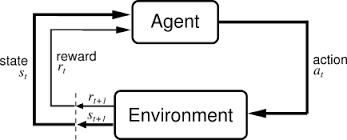
\includegraphics[width=0.5\textwidth]{ReinforcementLearning.png}
\caption{The agent-environment interaction in reinforcement learning.}  \label{fig:RL_Agent_Env}
\end{figure}

\indent We would like that a state summarizes past sensations compactly, in a such a way that all relevant information is retained - \textit{Markov property}. If the state has Markov property,  that the environment's response at $t+1$ depends only on the state and action representation at $t$. If an environment has Markov property then its one-step dynamics enable us to predict the next state and expected next reward given the current state and action

\begin{equation}
\ma{Pr}\{R_{t+1} = r, S_{t+1} = s' | S_t, A_t\}
\end{equation}

\indent Reinforcement learning task that satisfies the Markov property us \textit{Markov Decision Process}(MDP). Given any state and action, $s$ and $a$, the probability of each possible next state $s'$ is

\begin{equation}
p(s'| s, a) = \ma{Pr}\{S_{t+1} = s' | S_t = s, A_t = a\}
\end{equation}

These are called \textit{transition probabilities}. Similarly, given any current state and action, $s$ and $a$, together with any next state $s'$, the expected value of the next state reward is

\begin{equation}
r(s, a, s') =\expect[R_{t+1} | S_t = s, A_t = a, S_{t+1} = s']
\end{equation}

\subsubsection{Value functions}

Reinforcement learning algorithms involve estimating \textit{value functions} - functions of state or state-action pairs that estimate how good is for the agent to be in a given state or to perform a given action in a given state. It is defined in terms of future rewards that can be expected or in terms of expected return.
\\\\
\indent A policy $\pi$ is a mapping from each state $s \in \mathcal{S}$ and action $a \in \mathcal{A}(s)$ to the probability $\pi(a|s)$ of taking an action $a$ when in state $s$. The value of state $s$ under a policy $\pi$ - $v_{\pi}(s)$ is the expected return $G_t$ starting in state $s$ and following $\pi$ thereafter

\begin{equation}
v_{\pi}(s)=\expect_{\pi}[G_t | S_t = s] = \expect_{\pi}[\sum\limits_{k=0}^{\infty}\gamma^{k}R_{t+k+1}|S_t = s]
\end{equation}

where $\expect_{\pi}[\cdot]$ is the expected value given that the agent follows the policy $\pi$ and $v_{\pi}(s)$ is the \textit{state-value function} for policy $\pi$. $\gamma$ is \textit{discount rate}, $0 \leq \gamma \leq 1$, and it determines the present value of future rewards. A reward received $k$ time steps in the future worth only $\gamma^{k-1}$ times what it would be worth if it were received immediately.  
\\\\
\indent Similarly, we define the value of taking an action $a$ in state $s$ under policy $\pi$ denoted as $q_{\pi}(s,a)$ as the expected return starting from state $s$, taking an action $a$ and following the policy $\pi$ thereafter as:

\begin{equation}
q_{\pi}(s,a)=\expect_{\pi}[G_t | S_t = s, A_t = a] = \expect_{\pi}[\sum\limits_{k=0}^{\infty}\gamma^{k}R_{t+k+1}|S_t = s, A_t=a]
\end{equation}

\indent A fundamental property of value functions is that they satisfy recursive relationship:

\begin{align*}
v_{\pi}(s) &=\expect_{\pi}[G_t | S_t = s] \\
&= \expect_{\pi}[\sum\limits_{k=0}^{\infty}\gamma^{k}R_{t+k+1}|S_t = s] \\
&= \expect_{\pi}[R_{t+1} + \gamma\sum\limits_{k=0}^{\infty}\gamma^{k}R_{t+k+2}|S_t = s] \\
&=  \sum\limits_{a}\pi(a|s)\sum\limits_{s'}p(s'|s,a)[r(s,a,s') + \gamma\expect_{\pi}[\sum\limits_{k=0}^{\infty}\gamma^{k}R_{t+k+2}|S_{t+1} = s'] ]\\
&=  \sum\limits_{a}\pi(a|s)\sum\limits_{s'}p(s'|s,a)[r(s,a,s') + \gamma v_{\pi}(s')]
\end{align*}

This is is the \textit{Bellman equation} for $v_{\pi}$. It expresses a relationship between the value of a state and the values of its successor states.

\subsubsection{Optimal value functions}

Solving a reinforcement learning task means, roughly, finding a policy that achieves a lot of reward over the long run.  A policy $\pi$ is defined to be better than or equal to a policy $\pi'$ if its expected return is greater than or equal to that of $\pi'$ for all states. In other words, $\pi \geq \pi'$ if and only if $v_{\pi}(s) \geq v_{\pi}(s')$ for all $s\in \mathcal{S}$. There is always at least one policy that is better than or equal to all other policies. This is an optimal policy. Although there may be more than one, we denote all the optimal policies by $\pi_{*}$. They share the same state-value function, called \textit{optimal state-vale function} - $v_{*}$ defined as 

\begin{equation}
v_{*}(s) = \max_{\pi}v_{\pi}(s) 
\end{equation}

for all $s\in \mathcal{S}$. Optimal policies also share the same \textit{optimal action-value function} denoted as $q_{*}$ and defined as

\begin{equation}
q_{*}(s,a) = \max_{\pi}q_{\pi}(s,a) 
\end{equation}

for all $s \in \mathcal{S}$ and all $a \in \mathcal{A}(s)$. For all state-action pairs $(s,a)$ this function gives the expected return for taking an action $a$ in state $s$ and following the optimal policy thereafter. We can write $q_{*}$ in terms of $v_{*}$ as

\begin{equation}
q_{*}(s,a) = \expect[R_{t+1} + \gamma v_{*}(S_{t+1}) | S_t = s, A_t = a]
\end{equation}

Bellman optimality equation expresses the fact that the value of a state under an optimal policy must equal expected return for the best action from that state:

\begin{align*}
v_{*}(s) &=\max_{a \in \mathcal{A}(s)}q_{\pi_{*}}(s,a) \\
&= \max_{a}\expect_{\pi_{*}}[G_t | S_t = s, A_t = a] \\
&= \max_{a}\expect_{\pi_{*}}[\sum\limits_{k=0}^{\infty}\gamma^{k}R_{t+k+1}|S_t = s, A_t = a] \\
&= \max_{a}\expect_{\pi_{*}}[R_{t+1} + \gamma\sum\limits_{k=0}^{\infty}\gamma^{k}R_{t+k+2}|S_t = s, A_t = a] \\
&=  \max_{a}\expect[R_{t+1} + \gamma v_{*}(S_{t+1})| S_t = s, A_t = a]\\
& =  \max_{a}\sum\limits_{s'}p(s'|s,a)[r(s,a,s') + \gamma v_{*}(s')]
\end{align*}

The Bellman optimality equation for $q_{*}$ is
\begin{align*}
q_{*}(s,a) &=\expect[R_{t+1}+ \gamma \max_{a}q_{*}(S_{t+1},a')|S_t = s, A_t = a] \\
&=  \sum\limits_{s'}p(s'|s,a)[r(s,a,s') + \gamma \max_{a}q_{*}(s',a')]
\end{align*}


The objective of reinforcement learning is to maximize the amount of rewards agent receives over time. A policy's value functions assign to each state, or state-action pair, the expected return from that state, or state-action pair, given that the agent uses the policy. The optimal value functions assign to each state, or state-action pair, the largest expected return achievable by any policy. A policy whose value functions are optimal is an optimal policy. Whereas the optimal value functions for states and state-action pairs are unique for a given MDP, there can be many optimal policies.
\\\\
\color{red} How to define the model for reinforcement learning is still unknown to me since it depends on the results obtained in the previous papers. In general, in our case, states would represent the desk illuminance that depend on many environmental factors. This is the reason why we want to do feature/variable selection, to reduce the number of possible states, by finding only relevant ones. The actions represent user's control actions (changing a position of the slider from 0-100\%) and rewards can be defined in terms of deviation from user's preferred illuminance level. Depending on the results of the previous paper described in Section \ref{sec:FeaturePreference}, that will show us whether users define their preference in terms of output of the luminaire or desk illuminance, we can define action preference or state preference and try to optimize for one of them. An action preference $(s, a_1) > (s, a_2)$ means that it is preferred to select action $a_1$ opposed to $a_2$, when in state $s$.  A state preference $s_1>  s_2$ means that it is preferred to visit state $s_1$ opposed to state $s_2$. 
\\
\indent Furthermore, we can apply Mathys's approach for solving our problem, but we can discuss this.

\color{black}
\begin{itemize}
	\item{Based on the data from Study 2016}
	\begin{itemize}
		\item Envisioned journals:
			\begin{itemize}
				\color{blue}
				\item To be determined
			\end{itemize}
	\end{itemize}
\end{itemize}





%%%%%%%%%%%%%%%%%%%%%%%%%%%%%%%%%%%%%%%%%%
%%%%%%%%%%%%%%%%%%%%%%%%%%%%%%%%%%%%%%%%%%
\section {\color{gray}How knowing the context can help us even further (optional)}

The following chapters are optional, if we want to include previously published papers related to activity recognition and for showing how we can optimize energy in different cases. 

%%%%%%%%%%%%%%%%%%%%%%%%%%%%%%
\subsection{\color{gray}Activity recognition concept}

In this section we can present results obtained for activity recognition approach and show why how knowing the activities of the users can help us to optimize environmental conditions even further.

\begin{itemize}
	\item{\color{gray}Two conference papers from 2013}
\end{itemize}

%%%%%%%%%%%%%%%%%%%%%%%%%%%%%%%%
\subsection{\color{gray}Energy saving in office buildings}

In the following subsections we define and compare possible energy savings based on activity recognition approach and standards, if we have pure manual personal control over lighting and if we know users' lighting profiles.

%--------------------------------------------------------------------------------------------------------------
\subsubsection{\color{gray}Energy saving based on activity recognition and standards}

In this section we present possible energy savings by knowing activities of the users. For example, lighting should be dimmed if user performs computer-based tasks vs. desk-based tasks. The standards provide guidelines for illuminance levels based on these tasks. These calculations are already done in two conference papers that I published.

\begin{itemize}
	\item{\color{gray}Two conference papers from 2013}
\end{itemize}

%--------------------------------------------------------------------------------------------------------------
\subsubsection{\color{gray}Energy saving based on manual personal control}

In 2013 and 2014 studies, they compared energy consumption between different conditions: when the lights were held on fixed light level (approx. 500 lx on desks) vs. when users had manual personal control over lighting. In 2013 study, having personal control resulted in energy saving of 27.5\%. In 2014, there were 5 conditions and energy consumption was compared among them. The calculations for 2016 study still needs to be done.

\begin{itemize}
	\item{\color{gray}Based on Studies 2013,2014 and 2016}
\end{itemize}

%-------------------------------------------------------------------------------------------------
\subsubsection{\color{gray}Energy saving based on users' lighting profiles}

When we are able to derive preference profiles of the users, we can simulate how much energy we can save. The idea is that if for example, user's preference function can be modeled as some form of Gaussian function, we can derive the tolerance of the users as the deviation from his preferred illuminance level he is willing to accept without initiating a change/action. In one dimensional case, if we know the tolerance of the user, we can offer lighting which is $\mu - \sigma$, towards lower illuminance levels, where $\mu$ represents preferred illuminance level of a user, and $\sigma$ is the tolerance(deviation). The assumption is that user will not react in this case, but we can only perform a simulation, since we are unable to check it in a real test bed. 



\begin{itemize}
	\item{\color{gray}Based on Study 2016}
\end{itemize}


%%%%%%%%%%%%%%%%%%%%%%%%%%%%%%%%%%%%%
%%%%%%%%%%%%%%%%%%%%%%%%%%%%%%%%%%%%%
\section{Conclusions}







\end{document}